% Document class and parameters %
\documentclass[10pt,a4paper]{article}

% Document packages %
\usepackage{graphicx}
\usepackage{biblatex}
\usepackage{parskip}
\usepackage{listings}
\usepackage{caption}
\usepackage{subcaption}
\usepackage{amsmath}
\usepackage{amssymb}
\usepackage[most]{tcolorbox}
\usepackage{wrapfig}


% Parameters %
\lstset{basicstyle=\ttfamily, breaklines = true, tabsize=2}
\graphicspath{{./Images/}}
\setlength{\parskip}{1em}

% Document Body %
\begin{document}
\begin{titlepage}
	\centering
	{\scshape\LARGE Imperial College London \par}
	\vspace{1cm}
	{\scshape\Large Mathematics: Year 2\par}
	\vspace{1.5cm}
	{\huge\bfseries Vectors (1st Year)\par}
	\vspace{2cm}
	{\Large\ Xin Wang }
	\vfill
	{\large \today\par}
\end{titlepage}

\begin{abstract}
Vector notation is essential in the analysis of forces on a particular engineering system. This
later grew to include modelling multi-dimensional simulations.
\end{abstract}

\tableofcontents
\pagebreak

%%%%%%%%%%%%%%%%%%%%%%%%%%%%%%%%%%%%%%%%%%%%%%%%%%%%%%%%%%%%%%%%%%%%%%%%%%%%%%%%%%%%%%%%%%%%%%%%%%%%%%%%%%
% Sections Body %
\section{Vectors}
%%%%%%%%%%%%%%%%%%%%%%%%%%%%%%%%%%%%%%%%%%%%%%%%%%%%%%%%%%%%%%%%%%%%%%%%%%%%%%%%%%%%%%%%%%%%%%%%%%%%%%%%%%
\subsection{Basic definitions of vectors}

\begin{itemize}
    \item Vector addition and scalar multiplication satisfies the following properties:
    \begin{itemize}
        \item $\textbf{\underline{x}} + \textbf{\underline{y}} = \textbf{\underline{y}} + \textbf{\underline{x}}$
        \item $(\textbf{\underline{x}}+\textbf{\underline{y}})+\textbf{\underline{z}} =
        \textbf{\underline{x}} + (\textbf{\underline{y}}+\textbf{\underline{z}})$
        \item $\lambda(\textbf{\underline{x}}+\textbf{\underline{y}})=\lambda\textbf{\underline{x}} + \lambda\textbf{\underline{y}}$
        \item $(\lambda+\mu)\textbf{\underline{x}} = \lambda\textbf{\underline{x}} + \mu\textbf{\underline{x}}$
        \item $\mu(\lambda \textbf{\underline{x}})=(\mu\lambda)\textbf{\underline{x}}$
        \item $1\times\textbf{\underline{x}} = \textbf{\underline{x}}$ and $0\times
        \textbf{\underline{x}} = 0$
    \end{itemize}
\end{itemize}

%%%%%%%%%%%%%%%%%%%%%%%%%%%%%%%%%%%%%%%%%%%%%%%%%%%%%%%%%%%%%%%%%%%%%%%%%%%%%%%%%%%%%%%%%%%%%%%%%%%%%%%%%%
\subsection{Dot product}

\begin{itemize}
    \item Magnitude: $|\textbf{\underline{x}}| = \sqrt{\textbf{\underline{x}}}$
    \item Properties:
    \begin{itemize}
        \item $\textbf{\underline{x}}.\textbf{\underline{y}}=\textbf{\underline{y}}.\textbf{\underline{x}}$
        \item $\lambda(\textbf{\underline{x}}.\textbf{\underline{y}})=(\lambda
        \textbf{\underline{x}}).\textbf{\underline{y}}=\textbf{\underline{x}}.(\lambda
        \textbf{\underline{y}})$
        \item $\textbf{\underline{x}}.(\textbf{\underline{y}}+\textbf{\underline{z}})=\textbf{\underline{x}}.\textbf{\underline{y}}+\textbf{\underline{x}}.\textbf{\underline{z}}$
    \end{itemize}
    \item Orthogonality: $\textbf{\underline{x}}.\textbf{\underline{y}}=0$ 
    \item Angles: $\textbf{\underline{x}}.\textbf{\underline{y}}=|\textbf{\underline{x}}||\textbf{\underline{y}}|\cos(\theta)$
\end{itemize}

%%%%%%%%%%%%%%%%%%%%%%%%%%%%%%%%%%%%%%%%%%%%%%%%%%%%%%%%%%%%%%%%%%%%%%%%%%%%%%%%%%%%%%%%%%%%%%%%%%%%%%%%%%
\subsubsection{Projection}

\begin{itemize}
    \item Vector $\lambda \textbf{\underline{v}}$ is the \textbf{projection of
    $\textbf{\underline{u}}$ along direction vector $\textbf{\underline{v}}$}
    \item How much correlation $\lambda$: $\lambda = \frac{\textbf{\underline{u}}.\textbf{\underline{v}}}{\textbf{\underline{v}}.\textbf{\underline{v}}}$
\end{itemize}

%%%%%%%%%%%%%%%%%%%%%%%%%%%%%%%%%%%%%%%%%%%%%%%%%%%%%%%%%%%%%%%%%%%%%%%%%%%%%%%%%%%%%%%%%%%%%%%%%%%%%%%%%%
\subsubsection{Unit vector}

\begin{itemize}
    \item $\hat{\textbf{\underline{x}}} = \frac{1}{|\textbf{\underline{x}}|}=\textbf{\underline{x}}$
\end{itemize}

\pagebreak

%%%%%%%%%%%%%%%%%%%%%%%%%%%%%%%%%%%%%%%%%%%%%%%%%%%%%%%%%%%%%%%%%%%%%%%%%%%%%%%%%%%%%%%%%%%%%%%%%%%%%%%%%%
\subsection{Cross product}

\begin{itemize}
    \item Properties:
    \begin{itemize}
        \item $\textbf{\underline{a}}\times \textbf{\underline{b}}=-\textbf{\underline{b}}\times \textbf{\underline{a}}$
        \item $\textbf{\underline{a}}\times \textbf{\underline{a}}=0$
        \item $\lambda(\textbf{\underline{a}}\times \textbf{\underline{b}})=(\lambda
        \textbf{\underline{a}})\times \textbf{\underline{b}}=\textbf{\underline{a}}\times (\lambda
        \textbf{\underline{b}})$
        \item $\textbf{\underline{a}}.(\textbf{\underline{a}} \times \textbf{\underline{b}}) =
        \textbf{\underline{b}}.(\textbf{\underline{a}}\times \textbf{\underline{b}})=0$
        \item $\textbf{\underline{a}}\times
        (\textbf{\underline{b}}+\textbf{\underline{c}})=\textbf{\underline{a}}\times
        \textbf{\underline{b}}+\textbf{\underline{a}}\times \textbf{\underline{c}}$
    \end{itemize}
\end{itemize}

%%%%%%%%%%%%%%%%%%%%%%%%%%%%%%%%%%%%%%%%%%%%%%%%%%%%%%%%%%%%%%%%%%%%%%%%%%%%%%%%%%%%%%%%%%%%%%%%%%%%%%%%%%
\subsubsection{Shortest distance from point to plane}

\begin{itemize}
    \item Shortest distance is the perpendicular line between two vectors
    \begin{align*}
        d = \frac{|Ax_1+By_1+Cz_1 +D|}{\sqrt{A^2+B^2+C^2}}.
    \end{align*}
    where point $P=(x_1,y_1,z_1)$ and plane $Ax+By+Cz+D=0$
\end{itemize}

%%%%%%%%%%%%%%%%%%%%%%%%%%%%%%%%%%%%%%%%%%%%%%%%%%%%%%%%%%%%%%%%%%%%%%%%%%%%%%%%%%%%%%%%%%%%%%%%%%%%%%%%%%
\subsubsection{Distance between two lines}

\begin{itemize}
    \item Given two lines: $Ax + By + Cz + D_1 = 0$ and $Ax + By + Cz + D_2 = 0$:
    \begin{align*}
        d = \frac{|D_1 - D_2|}{\sqrt{A^2 + B^2 + C^2}}
    \end{align*}
\end{itemize}

%%%%%%%%%%%%%%%%%%%%%%%%%%%%%%%%%%%%%%%%%%%%%%%%%%%%%%%%%%%%%%%%%%%%%%%%%%%%%%%%%%%%%%%%%%%%%%%%%%%%%%%%%%
\subsubsection{Equation of a plane}

\begin{itemize}
    \item Given point $x$, normal $n$ and point on plane $r$, the equation:
    \begin{align*}
        (\textbf{\underline{r}}-\textbf{\underline{x}}).\textbf{\underline{n}} =0 
    \end{align*}
    \item $ Ax+By+Cz = D$ where:
    \begin{itemize}
        \item $\textbf{\underline{r}} = (x,y,z)$
        \item $\textbf{\underline{n}}=(A,B,C)$
        \item $D=\textbf{\underline{x}}.\textbf{\underline{n}}$
    \end{itemize}
    
\end{itemize}





%%%%%%%%%%%%%%%%%%%%%%%%%%%%%%%%%%%%%%%%%%%%%%%%%%%%%%%%%%%%%%%%%%%%%%%%%%%%%%%%%%%%%%%%%%%%%%%%%%%%%%%%%%
\subsubsection{Triple cross product}

\begin{itemize}
    \item Properties:
    \begin{itemize}
        \item Equal:
        \begin{align*}
            \textbf{\underline{a}}.(\textbf{\underline{b}}\times \textbf{\underline{c}})=\textbf{\underline{b}}.(\textbf{\underline{c}}\times \textbf{\underline{a}})=\textbf{\underline{c}}.(\textbf{\underline{a}}\times \textbf{\underline{b}})=-\textbf{\underline{a}}.(\textbf{\underline{c}}\times \textbf{\underline{b}})=-\textbf{\underline{b}}.(\textbf{\underline{a}}\times \textbf{\underline{c}})=-\textbf{\underline{c}}.(\textbf{\underline{b}}\times \textbf{\underline{a}})
        \end{align*}
        \item $\textbf{\underline{a}} \times (\textbf{\underline{b}}\times \textbf{\underline{c}})=(\textbf{\underline{a}}.\textbf{\underline{c}})\textbf{\underline{b}}-(\textbf{\underline{a}}.\textbf{\underline{b}})\textbf{\underline{c}}$
    \end{itemize}
\end{itemize}

\pagebreak

%%%%%%%%%%%%%%%%%%%%%%%%%%%%%%%%%%%%%%%%%%%%%%%%%%%%%%%%%%%%%%%%%%%%%%%%%%%%%%%%%%%%%%%%%%%%%%%%%%%%%%%%%%
\section{Matrix algebra}

%%%%%%%%%%%%%%%%%%%%%%%%%%%%%%%%%%%%%%%%%%%%%%%%%%%%%%%%%%%%%%%%%%%%%%%%%%%%%%%%%%%%%%%%%%%%%%%%%%%%%%%%%%
\subsection{Matrix multiplication}

\begin{itemize}
    \item Properties:
    \begin{itemize}
        \item $A(BC)=(AB)C$
        \item $(\lambda A)B=A(\lambda B)=\lambda(AB)$
        \item $(AB)^T = B^T A^T$
    \end{itemize}
\end{itemize}

%%%%%%%%%%%%%%%%%%%%%%%%%%%%%%%%%%%%%%%%%%%%%%%%%%%%%%%%%%%%%%%%%%%%%%%%%%%%%%%%%%%%%%%%%%%%%%%%%%%%%%%%%%
\subsection{Inverse}

\begin{itemize}
    \item $\textbf{\underline{x}}=A^{-1}\textbf{\underline{b}}$
\end{itemize}

%%%%%%%%%%%%%%%%%%%%%%%%%%%%%%%%%%%%%%%%%%%%%%%%%%%%%%%%%%%%%%%%%%%%%%%%%%%%%%%%%%%%%%%%%%%%%%%%%%%%%%%%%%
\subsection{Determinants}

\begin{itemize}
    \item $\text{det}(A) = ad-bc$
    \item $3\times 3$ matrix:
    \begin{figure} [h!]
        \centering
        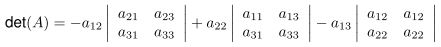
\includegraphics[scale=0.9]{Capture.JPG}
    \end{figure}
    \item Properties:
    \begin{itemize}
        \item The value of a determinant remains unchanged under transposition:
        \begin{align*}
            det(A) = det(A^T)
        \end{align*}
        \item If $B$ is obtained from $A$ by exchanging exactly two rows (or two columns)
        $$det(A) = -det(B)$$
        \item If the elements of any column (or row) are multiplied by a factor $\lambda$ then the determinant is multiplied by $\lambda$.
        \item If a multiple of one row (or column) is added to another row (or column), the determinant is unchanged.
        \item $det(AB) =det(A)det(B)$
    \end{itemize}
\end{itemize}
















%%%%%%%%%%%%%%%%%%%%%%%%%%%%%%%%%%%%%%%%%%%%%%%%%%%%%%%%%%%%%%%%%%%%%%%%%%%%%%%%%%%%%%%%%%%%%%%%%%%%%%%%%%
\end{document}